\documentclass[12pt,letterpaper]{article}
\usepackage{listings}
\usepackage{color}
\usepackage{textcomp}
\definecolor{listinggray}{gray}{0.9}
\definecolor{lbcolor}{rgb}{0.9,0.9,0.9}
\usepackage[utf8]{inputenc}
\lstset{
    language=SQL,
    basicstyle=\scriptsize,
    upquote=true,
    aboveskip={1.5\baselineskip},
    columns=fullflexible,
    showstringspaces=false,
    extendedchars=true,
    breaklines=true,
    showtabs=false,
    showspaces=false,
    showstringspaces=false,
    identifierstyle=\ttfamily,
    keywordstyle=\color[rgb]{0,0,1},
    commentstyle=\color[rgb]{0.133,0.545,0.133},
    stringstyle=\color[rgb]{0.627,0.126,0.941},
}

\usepackage[T1]{fontenc}

\usepackage[spanish]{babel}
\usepackage{amsmath}
\usepackage{amsfonts}
\usepackage{amssymb}
\usepackage{fancyhdr}
\usepackage{graphicx}
\usepackage{textcomp}
\usepackage{latexsym}
\usepackage{hyperref}
\usepackage[left=2cm, right=2cm, top=2cm, bottom=3.5cm]{geometry}
\begin{document}
\setlength{\unitlength}{1 cm} %Especificar unidad de trabajo
\thispagestyle{empty}
\begin{picture}(16,4)(0,0)
\put(0,0){
\includegraphics[width=5cm,height=3.5cm]{logos/logo_fcfm.jpg}}
\end{picture}
\\
\\
\\
\\
\\
\begin{center}
\textbf{{\Huge Tarea 2 }\\[4cm]
{\LARGE Modelo de Datos de una Red Social en BCNF}}\\[1cm]

{\Large Sebastián Hernández}\\[0.3cm]

CC3201 Bases de Datos
\\
Sección 1
\\
Profesor Jorge Perez
\\
Santiago, 21 de Octubre de 2013
\end{center}
\newpage
\pagestyle{fancy}
\headheight=60pt 					
\fancyhead[L]							
{	\begin{minipage}{6cm}
		
\includegraphics[width=0.9\textwidth]{logos/logo_DII.jpg}		
	\end{minipage}	}
\fancyhead[R]
{}
\setcounter{page}{1}
\tableofcontents

\newpage

\section{Introducción}
Para realizar esta tarea, se ofrecían dos opciones:

1. Puede comenzar desde sus tablas de la Entrega 1, definir todas las dependencias funcionales (y multivaloradas) que se deben cumplir y luego aplicar las técnicas de normalización para llevar su esquema al menos a BCNF.

2. Puede también empezar desde 0 creando un modelo Entidad/Vínculo completo de su dominio y luego aplicar alguno de los algoritmos vistos en clases para generar tablas. En este caso también deberá identificar las dependencias funcionales (y multivaloradas) que se deben cumplir y llevar su esquema al menos a BCNF.

En este trabajo se eligió la forma 1.

\section{Descripción del Problema}
Dominio 2: Red Social

Para este dominio debe crear una bases de datos y posteriormente una aplicación Web, capaz de manejar una red social basada en comentarios o reviews. La idea es que la red social le permita a usuarios casuales hacer comentarios de distintos recursos (libros, restaurantes, películas, etc.) y que permita también a analistas hacer estadísticas acerca de estos comentarios para clasificar los recursos y determinar el grado de aceptación o rechazo de estos.

Como en toda red social, los usuarios podrán interactuar con otros usuarios. En este caso los usuarios podrán tener amigos y también podrán seguir a otros usuarios cuando sus comentarios les parezcan interesantes. Adicionalmente los usuarios podrán decir cuándo un comentario ``les gusta'' o ``no les gusta'' (calidad del comentario) y podrán agregar etiquetas arbitrarias a los comentarios en la forma de palabras clave. Dado que se quiere mantener un conjunto razonable de palabras clave para cada comentario, los usuarios podrán también decir cuándo una palabra clave puesta por otro usuario les parece o no apropiada para el comentario.

Respecto de la relación entre comentarios, los usuarios podrán realizar comentarios sobre comentarios, comentarios sobre comentarios sobre comentarios, etc. al estilo de respuestas en un foro, para generar una discusión. Todas las características descritas en el párrafo anterior se aplican también a los comentarios supeditados a otros comentarios.

Note que la idea es que su base de datos y aplicación modele la interacción entre los usuarios de la red y la calidad de los comentarios. Por lo tanto sólo es necesario considerar de manera simple los datos asociados a los recursos que se están comentando.

Además de los detalles entregados, su base de datos debe contener al menos 8 atributos adicionales no mencionados en la anterior descripción. Estos atributos deben estar divididos entre atributos de los usuarios, atributos de los comentarios, etc.


Tipos de consultas que su sistema debe soportar 
Su interfaz final debe ser capaz de responder las siguientes consultas:

El comentario marcado con más ``me gusta''
Lista con información de los 5 usuarios que han obtenido la mayor cantidad de ``me gusta'' entre todos sus comentarios durante un mes específico del año.
Lista con las tres etiquetas que según los usuarios mejor describen un comentario dado
Para una etiqueta específica, cuál es el comentario con más ``me gusta''
Para una etiqueta específica, cuál es el comentario con más ``no me gusta''
Lista de los N usuarios con más amigos (donde N es un parámtero)
Lista de los N usuarios con más seguidores (donde N es un parámetro)
El usuario con más comentarios iniciales para un recurso
Información de los recursos que han sido más comentados
La cadena de comentarios con más respuestas
No es necesario que estas consultas sean respondidas en las primeras entregas y se incluyen sólo para guiar la construcción de sus tablas y los datos mínimos que deben contener.

\section{Solución}

A continuación se presenta la solución implementada para resolver el problema descrito. El siguiente esquema muestra todas las restricciones de llave primaria y foránea de las tablas, junto a sus restricciones de dominio. En el código anexo pueden verse en detalle todas estas restricciones.

\begin{figure}[hb]
  \centering
  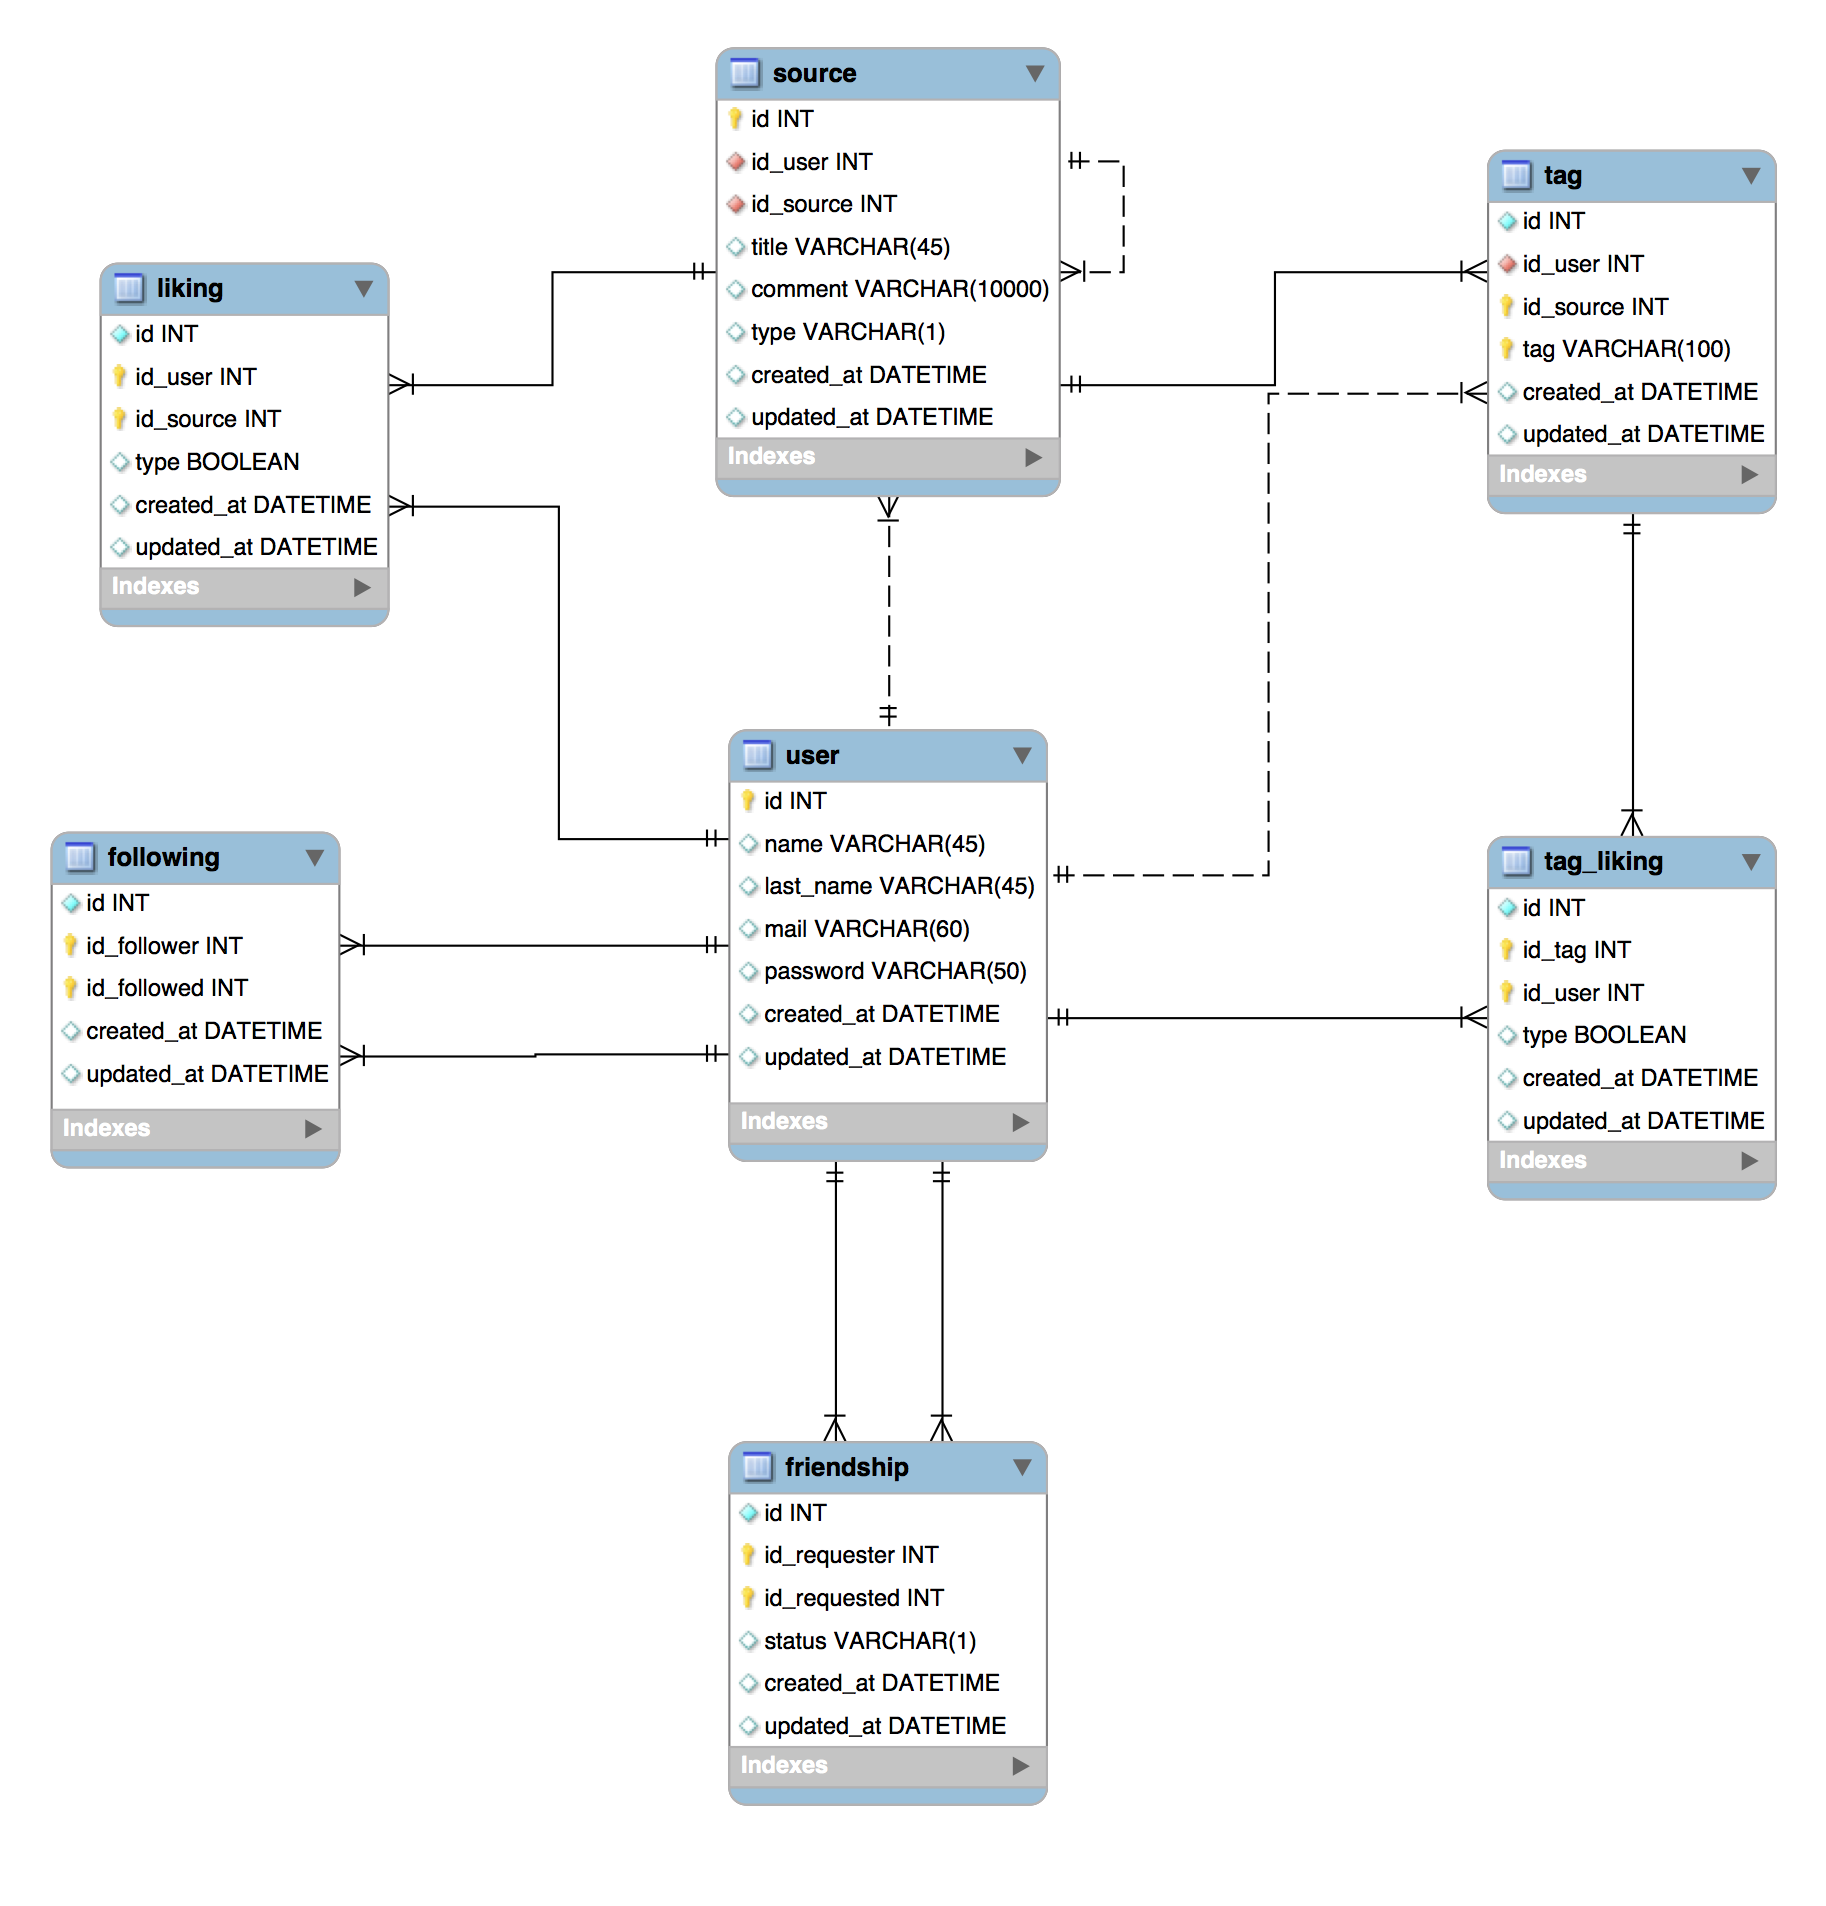
\includegraphics[scale=0.4]{images/modelo.png}
  \caption[Close up of \textit{Hemidactylus} sp.]
   {Esquema Entidad-Relación de la solución implementada.}
\label{fig:esquema}
\end{figure}



\subsection{Tabla User}
En la tabla Users se almacena la información de todos los usuarios que participan en la red social. Cada uno tiene un único ID, que se autoincrementa en 1 cada vez que un nuevo usuario es creado. El administrador de la base de datos no se tiene que preocupar por esto, es sólo para llevar la unicidad de cada usuario, de manera eficiente, ya que el mail puede ser muy largo, y eso implica espacio en la base de datos. El ID lo identifica de manera única. Además del ID, el mail también es único, es decir dos o mas usuarios no pueden tener el mismo mail. 
\begin{table}[!ht]  
\begin{center}	
	\begin{tabular}{||c|l|l|l|l|l|l|l|l|l|l|l||} \hline 
	id & name & last name & mail & password & created at & updated at \\ \hline
	\end{tabular}
	\caption {Tabla Users}
\end{center}  
\end{table}


\subsection{Tabla Source}
Esta tabla contiene los comentarios o recursos hechos por los usuarios. El atributo id user se encarga de identificar el usuario que ha realizado el comentario. El atributo title es usado sólo en caso de que el source sea de tipo recurso (r). El atributo type, revela el tipo de comentario o recurso que está realizando. Esto es, identifica si es un comentario hijo (comentario a otro comentario), comentario padre (primer comentario) o bien es un source. El atributo id source es el id del comentario o recurso padre en caso de que el comentario en cuestión sea un comentario hijo, y null si es un comentario padre o un source. 

\begin{table}[!ht]  
\begin{center}	
	\begin{tabular}{||c|l|l|l|l|l|l|l|l|l|l|l||} \hline 
	id & id user & id source & title & comment & type & created at & updated at \\ \hline
	\end{tabular}
	\caption {Tabla Comment}
\end{center}  
\end{table}

\subsection{Tabla Following}
En esta tabla se registra el seguimiento entre usuarios. El atributo id follower se encarga de identificar el usuario que está siguiendo a otro usuario, y este último es identificado por el atributo id followed. El registro de seguimiento es unidireccional, donde id follower sigue a id followed.

\begin{table}[!ht]  
\begin{center}	
	\begin{tabular}{||c|l|l|l|l|l|l|l|l|l|l|l||} \hline 
	id & id follower & id followed & created at & updated at \\ \hline
	\end{tabular}
	\caption {Tabla Following}
\end{center}  
\end{table}

\subsection{Tabla Friendship}
Esta tabla registra las peticiones de amistad, además del actual estado de ellas. El atributo id requester identifica al usuario que envió la petición de amistad, id requested identifica al usuario al que se le está invitando a una nueva amistad, status revela si la petición de amistad está pendiente, si fue rechazada o si fue aceptada, es decir, si actualmente son amigos.

\begin{table}[!ht]  
\begin{center}	
	\begin{tabular}{||c|l|l|l|l|l|l|l|l|l|l|l||} \hline 
	id & id requester & id requested & status & created at & updated at \\ \hline
	\end{tabular}
	\caption {Tabla Friendship}
\end{center}  
\end{table}

\subsection{Tabla Liking}
El atributo id user se encarga de identificar al usuario que realizó la declaración de aceptación o rechazo, y el atributo id source corresponde al id del source al que se aplica este like. El atributo type, indica el valor de aprobación, 0 si no le gusta, 1 si le gusta.

\begin{table}[!ht]  
\begin{center}	
	\begin{tabular}{||c|l|l|l|l|l|l|l|l|l|l|l||} \hline 
	id & id user & id source & type & created at & updated at \\ \hline
	\end{tabular}
	\caption {Tabla Liking}
\end{center}  
\end{table}

\subsection{Tabla Tag}
Esta tabla se encarga de guardar las diferentes etiquetas a los diferentes recursos o comentarios. El atributo id user identifica al usuario que creó la etiqueta y id source corresponde al id del source al que se le está aplicando el tag. El, atributo tag corresponde a la etiqueta en sí.

\begin{table}[!ht]  
\begin{center}	
	\begin{tabular}{||c|l|l|l|l|l|l|l|l|l|l|l||} \hline 
	id & id user & id source & tag & created at & updated at \\ \hline
	\end{tabular}
	\caption {Tabla Tag}
\end{center}  
\end{table}

\subsection{Tabla Tag Liking}
Esta tabla registra la aprobación o rechazo que tienen los diferentes usuarios para diferentes etiquetas. El atributo id user identifica al usuario que aprueba o rechaza una etiqueta, id tag identifica a la etiqueta que está siendo valorada, y type el valor de dicha aprobación: 0 si no le gusta, 1 si le gusta.

\begin{table}[!ht]  
\begin{center}	
	\begin{tabular}{||c|l|l|l|l|l|l|l|l|l|l|l||} \hline 
	id & id tag & id user & type & created at & updated at \\ \hline
	\end{tabular}
	\caption {Tabla Tag Liking}
\end{center}  
\end{table}


\section{Dependencias funcionales}

Las dependencias funcionales se muestran en el esquema de la Figura~\ref{fig:esquema}.

\section{Consultas SQL}

La consulta 1: Si se desea saber cuán popular es cada un usuario, ordenados de más popular, a menos.
La consulta 2: Si se desea enlistar y empaginar todos los comentarios, guardando el orden de prioridad para aquellos que comentarios padres que hayan sido comentados. En dicho caso, ese comentario padre es 'fresco' porque fué recientemente comentado, es decir su updates at fue modificado. Esta consulta cumplirá dicha función. Hay que tener cuenta solamente lo que ponemos en LIMIT. El primer atributo del LIMIT es primer el número de página, menos uno, multiplicado por la cantidad de comentarios que se desea enlistar por cada página. El segundo atributo corresponde a la cantidad de comentarios que se desea enlistar por cada página


\section{Anexo}
\subsection{Estructura de Tablas de la Base de Datos}




\end{document}
